\newpage

\section*{ $^{103}$Rh(n,n')$^{103m}$Rh }

Power Level: 100 kW(th) \\
Time at Power: 60.0 m \\
Wait Time: 60.0 m \\
Counting Time: 30.0 m \\
Total Activity at Removal: 4.49e+03 $\mu Ci$

\begin{table*}[h]
\centering
\begin{tabular}{ |c|c|c|c|c|c| }
 \hline
 Position & Mass $mg$ & Counting Activity $\mu Ci$ & Area (Counts) & Error \% \\
 \hline 
 1 & 7.40 & 9.57e+02 & 6.99e+04 & 0.3782 \\ 
\hline
 2 & 7.40 & 1.06e+03 & 7.71e+04 & 0.3601 \\ 
\hline
 3 & 7.40 & 6.57e+02 & 4.80e+04 & 0.4563 \\ 
\hline
 4 & 7.40 & 2.05e+02 & 1.50e+04 & 0.8177 \\ 
\hline
\end{tabular}
\end{table*}

\begin{figure}[h]
\centering
\begin{subfigure}{.5\textwidth}
  \centering
     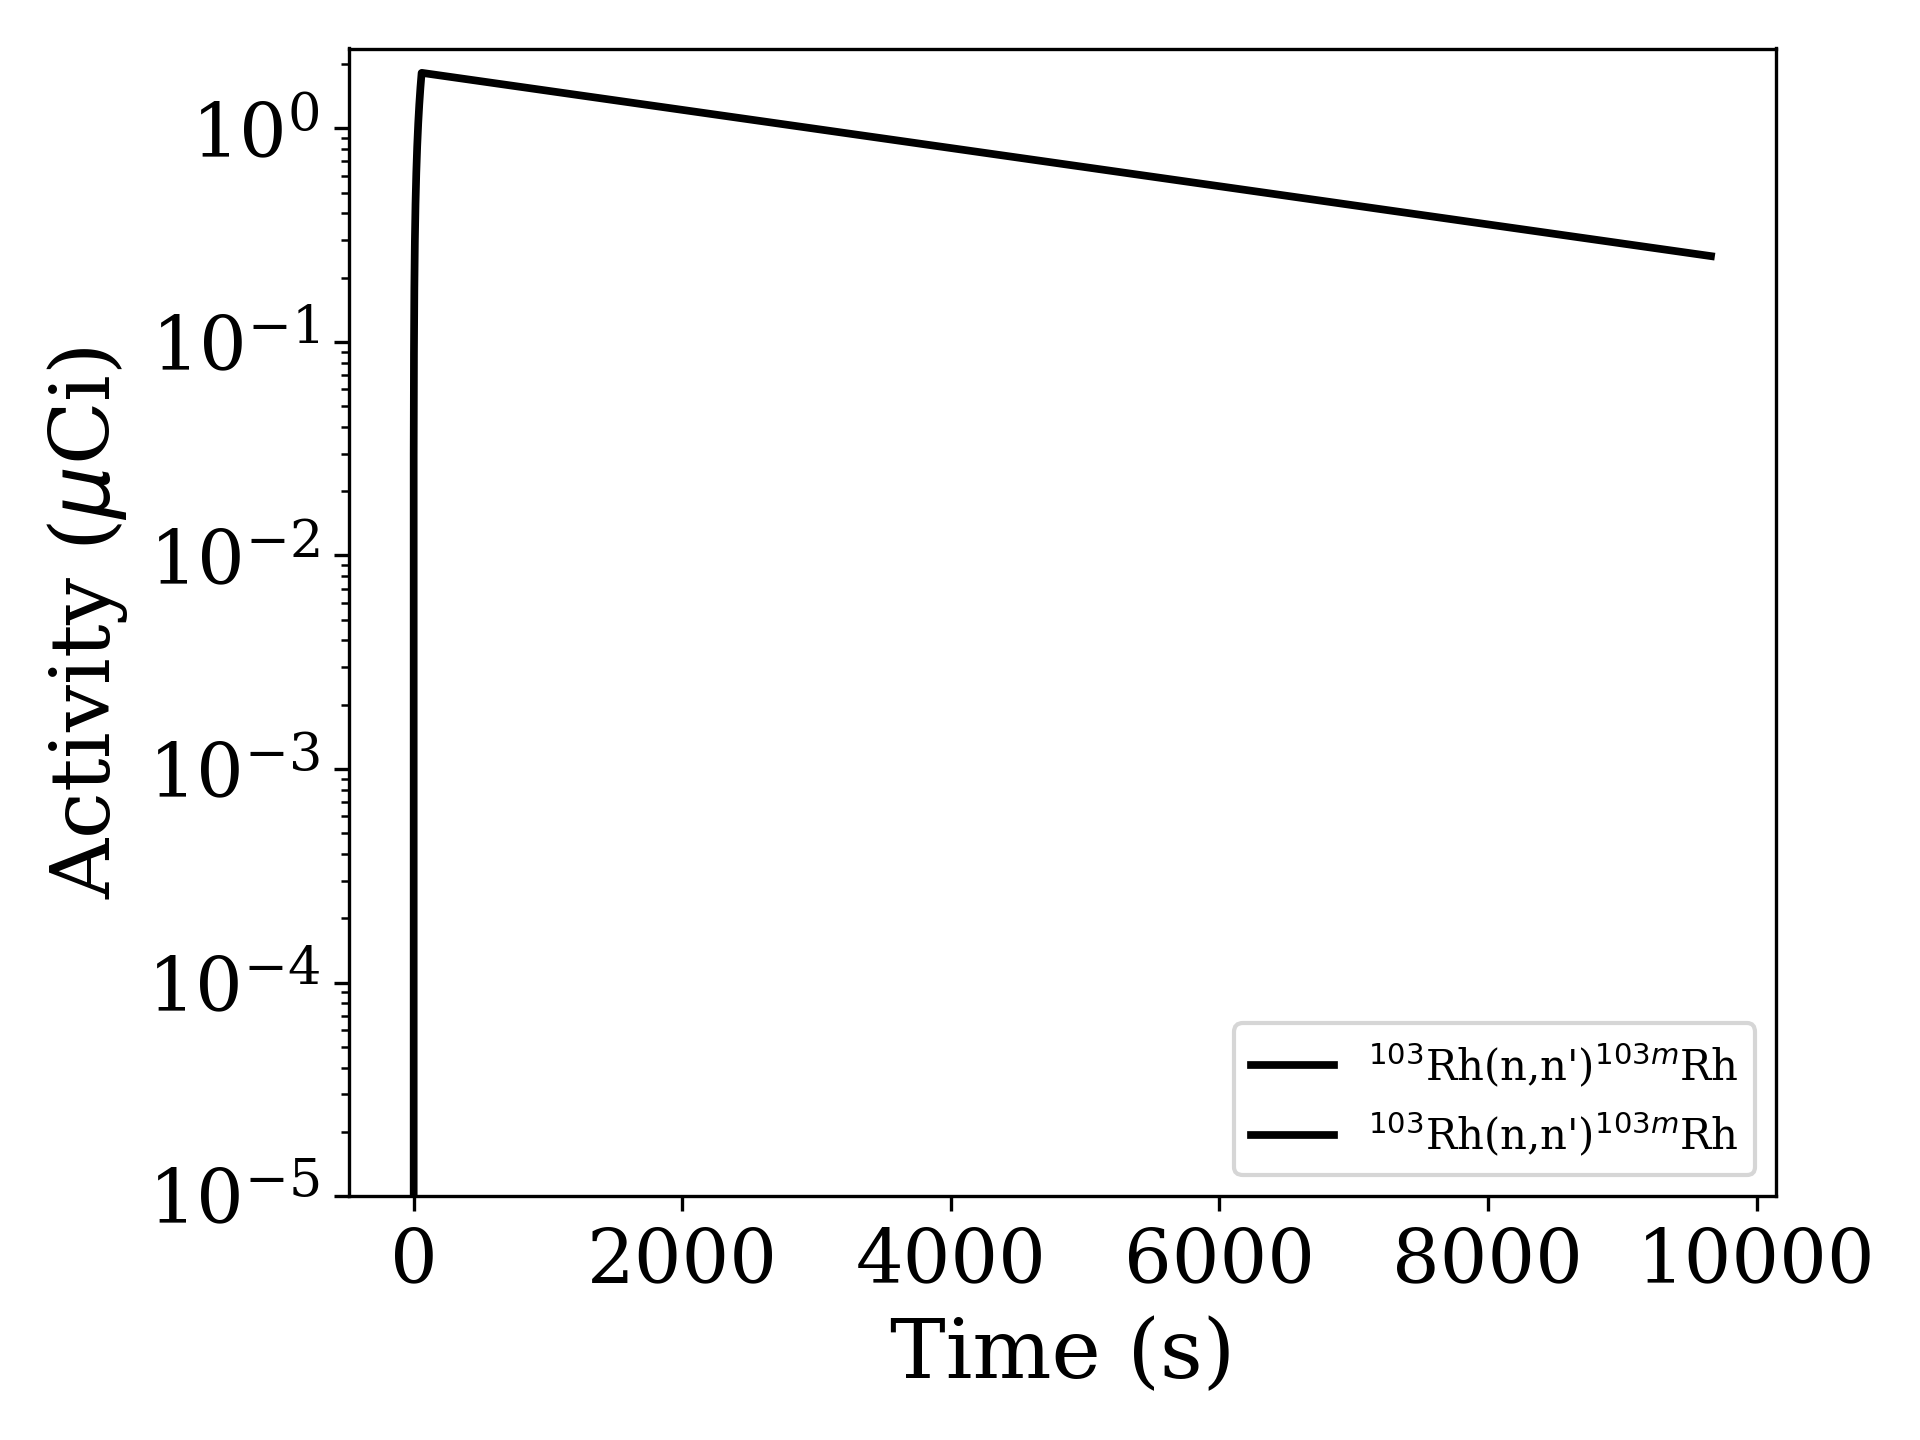
\includegraphics[width=.8\textwidth]{plot/Rh-103(n,n')Rh-103m_wisconsin1} 

  \caption{Activity}
\end{subfigure}%
\begin{subfigure}{.5\textwidth}
  \centering
     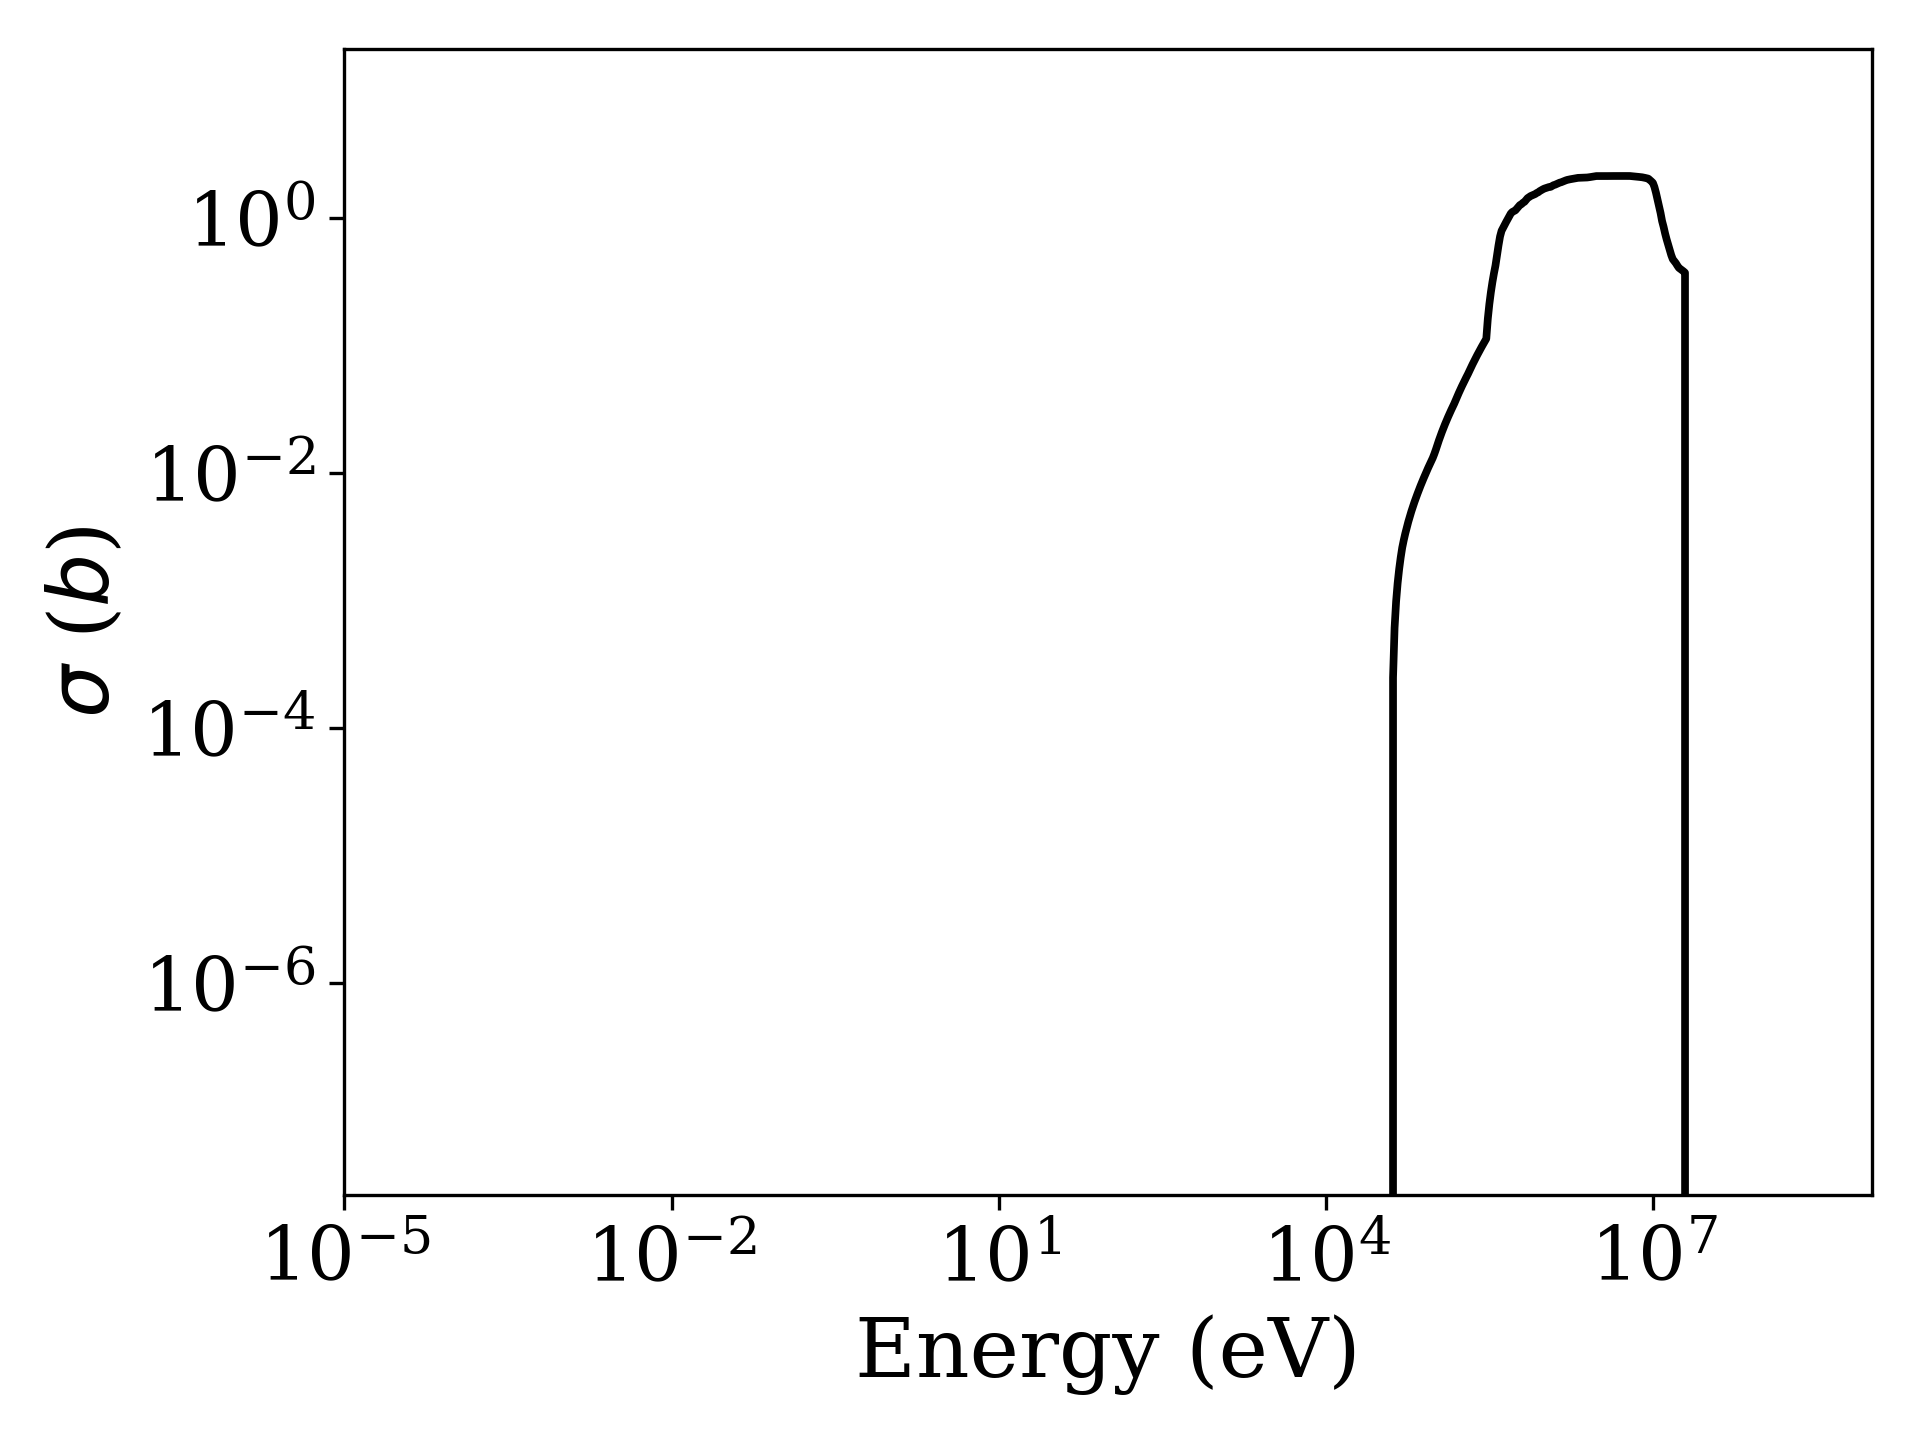
\includegraphics[width=.8\textwidth]{plot/Rh-103(n,n')Rh-103m} 

  \caption{Cross Section}
\end{subfigure}
\end{figure}

\begin{table*}[h]
\centering
\begin{tabular}{ |c|c|c|c|c|c|c| }
 \hline
 Reaction & T$_{1/2}$ & ROI (eV) & Important Gammas (keV) \\
 \hline 
 $^{103}$Rh(n,n')$^{103m}$Rh & 56.1 m & 4.91e+05, 5.21e+06 & 39.755(0.00068) \\ 
\hline
\end{tabular}
\end{table*}
